%Author: Martiano Jimenez
%Date: 30.December.2024

\documentclass[11pt]{beamer}
\usetheme{Darmstadt}
\usepackage[utf8]{inputenc}
\usepackage[spanish]{babel}
\usepackage{amsmath}
\usepackage{amsfonts}
\usepackage{amssymb}
\usepackage{graphicx}
\author{Ing. Mariano Jim\'enez Brenes}
\title
{
E2025C2-G01-ELECTRÓNICA DIGITAL Y SEMICONDUCTORES.
}
%\setbeamercovered{transparent} 
%\setbeamertemplate{navigation symbols}{} 
\logo{
\includegraphics[height=0.75cm]{./images/castrocarazo.eps}\vspace{5pt}} 
\institute{
Universidad Castro Carazo\linebreak
T\'ecnico En Semiconductores
} 
\date{Mi\'ercoles 14.Mayo.2025} 
%\subject{} 
\begin{document}

\begin{frame}
\maketitle 
\end{frame}

% Remove logo from the next slides
\logo{}

\begin{frame}
\frametitle{Contenido}
\tableofcontents
\end{frame}

\section{Complementos}
\begin{frame}{Complementos}
\frametitle{Complementos}
Las computadoras digitales usan complementos para simplificar la operaci\'on de resta.\linebreak
	\begin{itemize}
		\item Complemento a 1 de n\'umeros binarios.\linebreak
		$1101 \rightarrow 0010$
		\item Complemento a 2 de n\'umeros binarios.\linebreak
		$1101 \rightarrow 0011$
	\end{itemize}
\end{frame}
\subsection{Ejercicios}
\begin{frame}{Ejercicios de Complementos}
	\frametitle{Ejercicios de Complementos}
Realice los ejercicios 1.18, 1.20 del libro Morris Mano.
	\end{frame}

\section{C\'odigos Binarios}
\begin{frame}{C\'odigos Binarios}
\frametitle{C\'odigos Binarios}
A continuaci\'on se expondr\'an 4 tipos de c\'odigos:
	\begin{itemize}
		\item C\'odigo BCD.
		\item C\'odigo $2421$ y $Exceso-3$.
		\item C\'odigo Gray.
		\item C\'odigo ASCII.
		\item C\'odigos para detectar errores.\linebreak
		
		\begin{tabular}{ c c c }
		  					& \textbf{Paridad Par} & \textbf{Paridad Impar} \\ 
		 ASCII A = $1000001$ & $01000001$ & $11000001$ \\  
		 ASCII T = $1010100$ & $11010100$ & $01010100$    
		\end{tabular}
		
	\end{itemize}
\end{frame}

\subsection{Ejercicios}
\begin{frame}{Ejercicios de C\'odigos Binarios}
\frametitle{Ejercicios de C\'odigos Binarios}
Realice los ejercicios 1.22, 1.25 del libro Morris Mano.
\end{frame}

\section{Registros}
	\begin{frame}{Registros}
		\frametitle{Registros}
Una celda binaria es un dispositivo que tiene 2 estados estables y puede almacenar un bit de informaci\'on. Siguiendo esta idea, un registro es un grupo de celdas binarias cuyo contenido es función de la interpretaci\'on que se da a la informaci\'on ah\'i almacenada.
	\end{frame}
	
	\begin{frame}{Transferencia de Registros}
		\frametitle{Transferencia de Registros}
		\begin{columns}
			\column{0.3\linewidth}
				\begin{figure}[h]
					\centering
					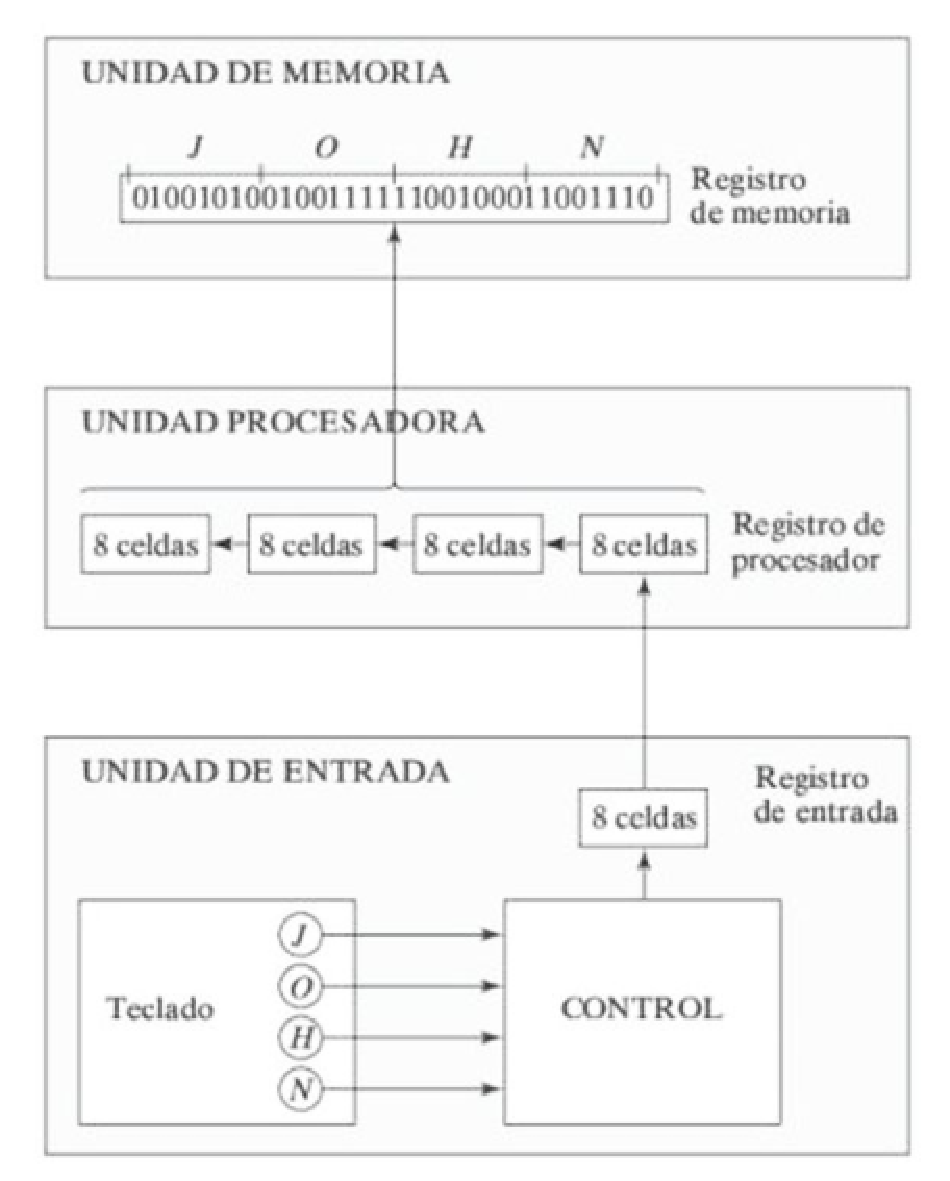
\includegraphics[height=5.0cm]{./images/transfer.eps}\vspace{1pt}
				\end{figure}
			\column{0.7\linewidth}
				\begin{itemize}
					\item En la unidad de entrada, una tecla podr\'ia transmitir su c\'odigo de manera serial o paralela.
					\item La unidad de control podr\'ia esperar una cantidad definida de caracteres o esperar por un c\'odigo en espec\'ifico.
					\item La unidad procesadora podr\'ia utilizar alguno de los c\'odigos binarios vistos anteriormente, inclusive, detectar alg\'un error proveniente del teclado.
					\item La unidad de memoria posee una cantidad finita de registros y cada registro se asocia con una direcci\'on.
				\end{itemize}
		\end{columns}
	\end{frame}

\section{L\'ogica Binaria}
	\begin{frame}{L\'ogica Binaria}
		\frametitle{L\'ogica Binaria}
		Esencialmente la l\'ogica binaria se compone de:
		\begin{itemize}
			\item Variables binarias
			\item Tres operadores b\'asicos: $NAD$, $OR$ y $NOT$ \linebreak
		\end{itemize}
		%\linebreak
		¿Existe alguna similitud entre la Aritm\'etica Binaria y la L\'ogica Binaria?
	\end{frame}
	\subsection{Tablas de Verdad}
	\begin{frame}{Tablas de Verdad}
		\frametitle{Tablas de Verdad}
		\begin{figure}[h]
			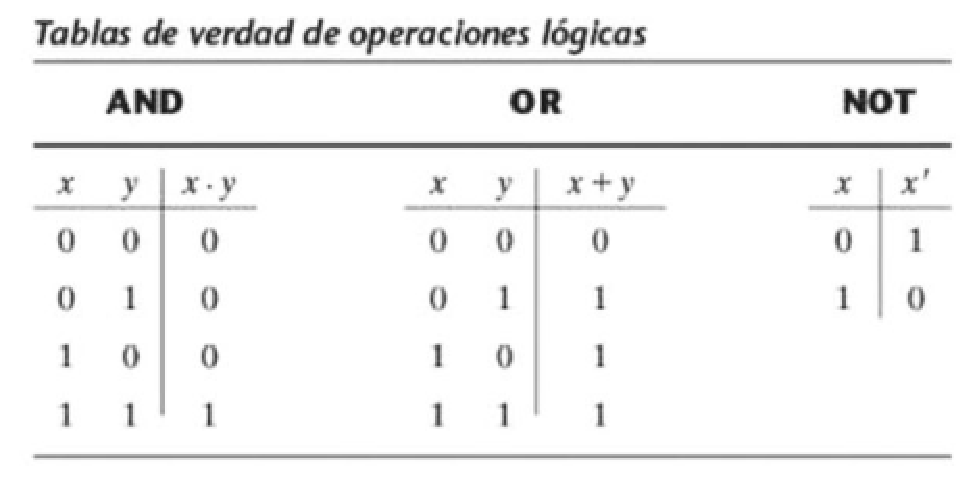
\includegraphics[height=3.0cm]{./images/tt.eps}\vspace{1pt}
		\end{figure}
	\end{frame}
	
	\subsection{Diagrama de Temporizaci\'on}
		\begin{frame}{Diagramas de Temporizaci\'on}
			\frametitle{Diagramas de Temporizaci\'on}
			\begin{figure}[h]
				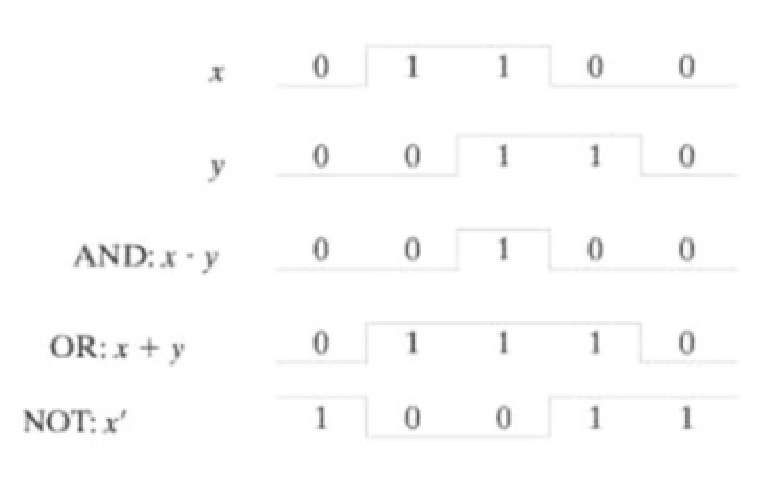
\includegraphics[height=3.0cm]{./images/td.eps}\vspace{1pt}
			\end{figure}
		\end{frame}	

	\subsection{Ejercicios}
		\begin{frame}{Ejercicios de C\'odigos Binarios}
		\frametitle{Ejercicios de C\'odigos Binarios}
			Realice los ejercicios 1.35, 1.36 del libro Morris Mano.
		\end{frame}
	
\section{Actividades Asincr\'onicas}
\begin{frame}
\frametitle{Actividades Asincr\'onicas}
	\begin{itemize}
		\item Portafolio: Conversiones Num\'ericas y diagramas de Temporizaci\'on.
		\item Indagaci\'on: Utilizando la AI investigue y comente en el foro una pequeña reseña sobre circuitos integrados lógica TTL, ECL, MOS, CMOS.
		\end{itemize}
\end{frame}

\section{Bibliograf\'ia}
\begin{frame}
	\frametitle{Bibliograf\'ia}
	\begin{itemize}
		\item Morris, M., y Ciletti, M. Diseño Digital, Cap. 1, pág. 11-33.
		\item Argüello D. M, Pérez, S., y Facchini, H. Arquitectura de computadoras, Cap.1, pág. 30-62.
		\end{itemize}
\end{frame}

\end{document}